\documentclass[11pt]{article}

%imports
\usepackage[utf8]{inputenc}
\usepackage[T1]{fontenc}
\usepackage{amsmath}
\usepackage{amsfonts}
\usepackage{amssymb}
\usepackage{footnote}
\usepackage{url}
\usepackage{hyperref}
\usepackage{subcaption}
\usepackage{multirow}


%images and image path
\usepackage{graphicx}
%\usepackage{subfig}
\graphicspath{ {./images/} }

%custom commands
\newcommand{\N}{\mathcal{N}}
\newcommand{\num}{\text{num}}
\newcommand{\obs}{\text{obs}}
\newcommand{\D}{\mathfrak{D}}
\newcommand{\Ro}{\mathcal{R}_0}
\newcommand{\lap}{{\mathcal{L}}}
\renewcommand\vec{\mathbf}
\newcommand{\mat}[1]{\mathsf{#1}}
\newcommand{\U}{\mathcal{U}}

%insitute command
\usepackage{etoolbox}
\makeatletter
\providecommand{\institute}[1]{% add institute to \maketitle
	\apptocmd{\@author}{\end{tabular}
	\par
	\begin{tabular}[t]{c}
		\small \textit{#1}}{}{}
}
\makeatother

%margins
\usepackage[letterpaper, total={6.5in, 9.5in}]{geometry}

%opening
\title{Reaction-diffusion spatial modeling of COVID-19 in Chicago}
\author{Trent Gerew\thanks{\texttt{tgerew@hawk.iit.edu}}}
\institute{Department of Applied Mathematics, Illinois Institute of Technology, Chicago, Illinois}

\begin{document}

\maketitle

	\begin{figure}[h]
		\centering
		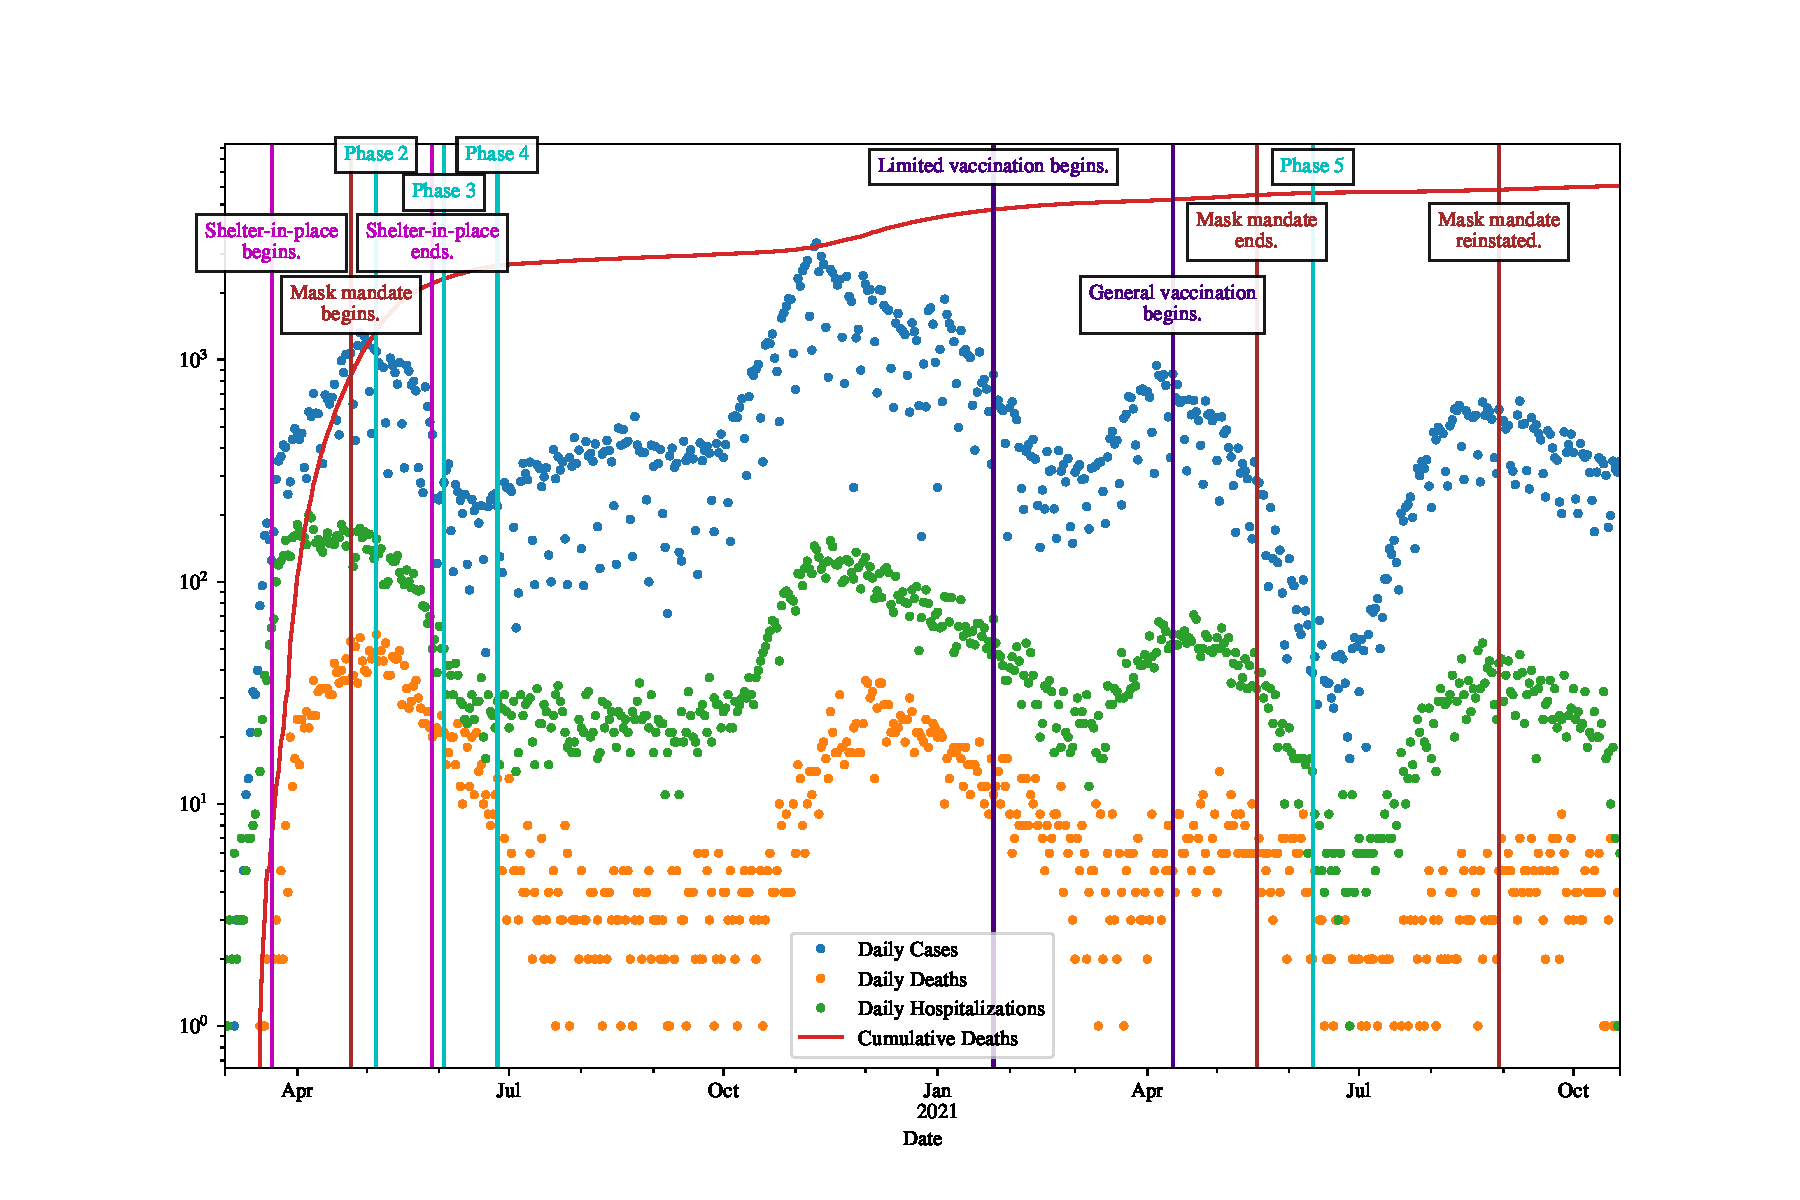
\includegraphics[height=12cm]{chicago-data2}
		\label{fig:data}
		\caption{Timeline of the progression of COVID-19 in Chicago with key public policy events marked.
			The COVID-19 data was obtained from the City of Chicago Data Portal \cite{Chicago-cases}.
			The dates of the policy events were gathered from the Illinois.gov press releases \cite{phase-5}, \cite{mask-lift}, \cite{full-vax}, \cite{start-vax}, \cite{phase-4}, the Chicago Tribune \cite{phase-3}, and NBC Chicago \cite{phase-2}.
			Note the logarithmic scale.}
	\end{figure}

\section{Model Setup}
	We begin by explaining the ODE model.
	This is obtained from the full PDE model in Equations (\ref{eq:s_t})-(\ref{eq:d_t}) by simply removing the diffusion terms.
	
	We extend the standard SIR model to incorporate key aspects of the COVID-19 virus.
	
	Given the time scale of the pandemic, we model a weak effect of the change in the susceptible population from births or other mortality factors with the term $- \mu S$.
	We estimate $\mu = 1.8997 \times 10^{-5}$ [per day] using the average United States death rate in urban regions from 2019 \cite{death-trends}.
	
	\begin{table}[h]
		\centering
		\caption{Time sequence of events and simulation times.}
		\label{tab:times}
		\begin{tabular}{ c c c c }
			\hline
			\hline
			Initial simulation time	&	Imposed lockdown	&	Effective lockdown	&	Last fitting day	\\
			\hline
			March 18, 2020	&	March 21, 2020	&	 April 1, 2020	&	June 24, 2020	\\
			$t_i = 1$	&	$t_q = 4$	&	$t_q = 15$	&	$t_f = 99$ \\
			\hline
			\hline
		\end{tabular}
	\end{table}
	
	\begin{figure}[h!]
		\centering
		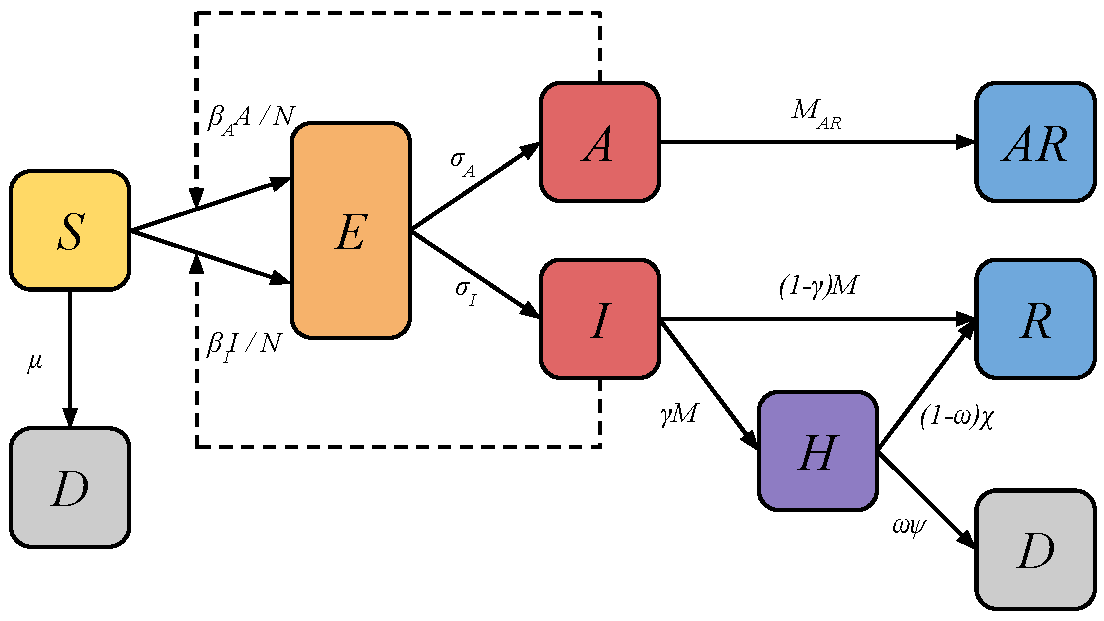
\includegraphics[height=6cm]{full-model}
		\label{fig:model}
		\caption{Schematic diagram of the model. The dashed lines indicate the interaction of the infected populations with the susceptible populations that leads to infection.}
	\end{figure}

	\begin{align}
		\label{eq:s_t}
		S_t &=	\D_S \Delta S - \beta_{SA} S A - \beta_{SI} S I - \mu S, \\
		\label{eq:e_t}
		E_t	&=	\D_E \Delta E + \beta_{SA} S A + \beta_{SI} S I - (\sigma_A + \sigma_I) E, \\
		\label{eq:ar_t}
		AR_t &= M_{AR} A, \\
		\label{eq:a_t}
		A_t	&=	\D_A \Delta A + \sigma_A E - M_{AR} A, \\
		\label{eq:i_t}
		I_t	&=	\sigma_I E - M I, \\
		\label{eq:h_t}
		H_t	&=	\gamma M I - (1 - \omega) \chi H - \omega \psi H, \\
		\label{eq:r_t}
		R_t	&=	(1 - \gamma) M I + (1 - \omega) \chi H, \\
		\label{eq:d_t}
		D_t	&=	\omega \psi H.
	\end{align}
	
	To create the PDE model, we first must find suitable parameters using the ODE model as in previous studies.
	We utilize the MATLAB nonlinear optimization algorithm \verb|fminsearch| for this purpose.
	The optimal parameters are determined by minimizing the Euclidean distance $\mathcal{N}$ between the time series generated by the model (subscript ``num'') and the corresponding observed data time series (subscript ``obs'')
	\begin{equation} \label{eq:objfun}
		\mathcal{N} = \sum_i \left( \left| \ln C_\mathrm{num} (t_i) - \ln C_\mathrm{obs} (t_i) \right| + \left| \ln D_\mathrm{num} (t_i) - \ln D_\mathrm{obs} (t_i) \right| \right)
	\end{equation}
	where the index $i$ identifies a point in the time series.
	The parameters are chosen to reproduce the time series of the total number of cases $C(t) = I(t) + H(t) + R(t) + D(t)$, and the total number of deceased $D(t)$.
	
	\begin{table}[h]
		\centering
		\caption{Population values for Chicago.
			Initial populations are determined from March 13, 2020.}
		\label{tab:populations}
		\begin{tabular}{ c c c }
			\hline
			\hline
			&	&	Population \\
			\hline
			Total population		&	$N$		&	2,695,598 \\
			Initial infected		&	$I_0$	&	162	\\
			Initial hospitalized	&	$H_0$	&	38 \\
			Initial deceased		&	$D_0$	&	3 \\
			\hline
			\hline
		\end{tabular}
	\end{table}

	To account for changes in virus transmission due to the shelter-in-place order, we impose a time dependence on the transmission rates $\beta$ as in Equations (\ref{eq:beta-si}) and (\ref{eq:beta-sa}).
	\begin{align}
		\label{eq:beta-si}
		\beta_{SI} (t) &= \beta_{SI} \left( \eta_{SI} + (1 - \eta_{SI}) \frac{1 - \tanh [2(t - t_q)]}{2} \right) \\
		\label{eq:beta-sa}
		\beta_{SA} (t) &= \beta_{SA} \left( \eta_{SA} + (1 - \eta_{SA}) \frac{1 - \tanh [2(t - t_q)]}{2} \right)
	\end{align}
	
	\begin{table}[h]
		\centering
		\caption{ODE parameters: optimal (best-fitting), median and interquartile range, and variation range used in the optimization algorithm.
			Initial parameter guesses were uniformly sampled within these ranges.}
		\label{tab:parameters}
		\begin{tabular}{ c c c c }
			\hline
			\hline
																								&					&	Median (IQR)	&	Initial value \\
			\hline
			Transmission rate, $S \to I$ [per day]\textsuperscript{a}							&	$\beta_{SI}$	&									&	$c \in \U [0,1]$ \\
			Transmission rate, $S \to A$ [per day]\textsuperscript{a}							&	$\beta_{SA}$	&									& 	$c \in \U [0,1]$ \\
			Lockdown effect, $S \to I$															&	$\eta_{SI}$ 	&									& 	$c \in \U [0,1]$ \\
			Lockdown effect, $S \to A$															&	$\eta_{SA}$		&									& 	$c \in \U [0,1]$ \\
			Incubation period, $E \to I$ [days]													&	$1 / \sigma_I$	&									& 	$1 / k, k \in \U [2,7]$ \\
			Latent period, $E \to A$ [days]														&	$1 / \sigma_A$	&									& 	$1 / k, k \in \U [2,7]$ \\
			Infectivity period [days]															&	$1 / M$			&									& 	$1 / k, k \in \U [5,12]$ \\
			Recovery period, $A \to AR$ [days]													&	$1 / M_{AR}$	&									& 	$1 / k, k \in \U [5,12]$ \\
			Recovery period, $H \to R$ [days]													&	$1 / \chi$		&									& 	$1 / k, k \in \U [5,20]$ \\
			Period to deceased, $H \to D$ [days]												&	$1 / \psi$		&									& 	$1 / k, k \in \U [5,20]$ \\
			Conversion fraction $(I \xrightarrow{\gamma} H, \ I \xrightarrow{1 - \gamma} R)$	&	$\gamma$		&									& 	$c \in \U [0.25,0.75]$ \\
			Conversion fraction $(H \xrightarrow{\omega} D, \ H \xrightarrow{1 - \omega} R)$	&	$\omega$		&									& 	$c \in \U [0.1,0.5]$ \\
			Initial population fraction, exposed												&	$E_0 / I_0$		&									& 	$c \in \U [1,5]$ \\
			Initial population fraction, asymptomatic											&	$A_0 / I_0$		&									& 	$c \in \U [1,5]$ \\
			\hline
			\hline
			\multicolumn{4}{c}{\small \textsuperscript{a} Note: The transmission rates $\beta$ must be divided by $N$ when used in the ODE model.}
		\end{tabular}
	\end{table}

	\begin{figure}[h!]
		\centering
		\begin{subfigure}{0.5\textwidth}
			\centering
			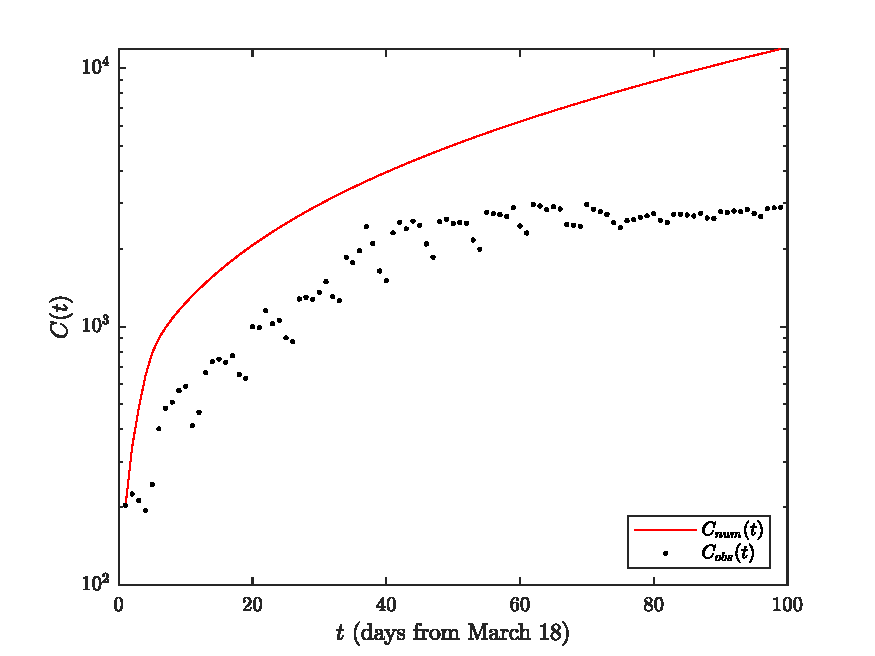
\includegraphics[height=6cm]{cases}
			\label{fig:ode-cases}
			\caption{Confirmed cases $C(t) = I(t) + R(t) + H(t) + D(t)$.}
		\end{subfigure}%
		\begin{subfigure}{0.5\textwidth}
			\centering
			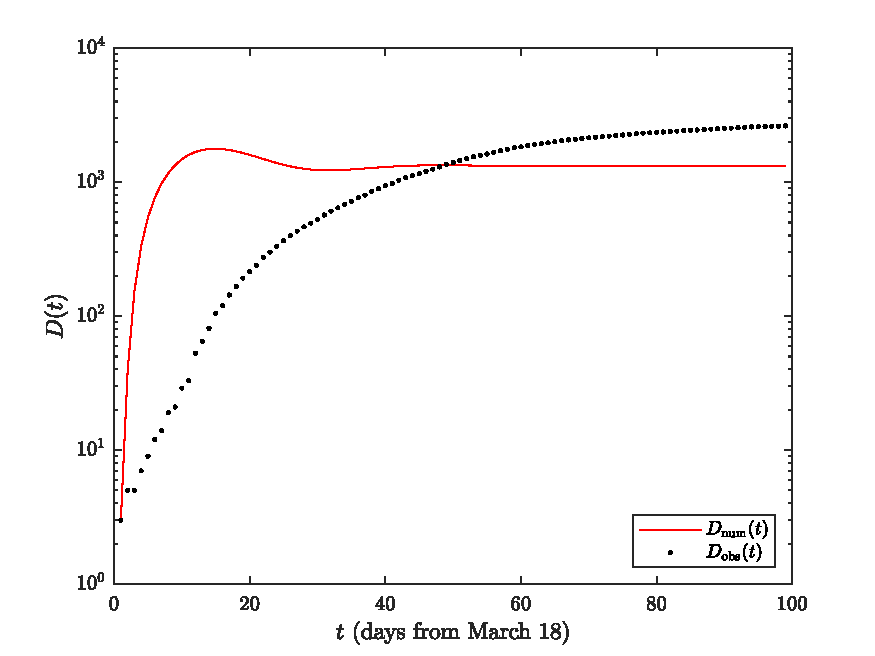
\includegraphics[height=6cm]{deaths}
			\label{fig:ode-deaths}
			\caption{Number of deaths $D(t)$.}
		\end{subfigure}
		\caption{ODE model with fitting to official data from March 18, 2020 ($t_i = 1$) to June 24, 2020 ($t_f = 99$).
		Here we show the case when $\beta$ changes exactly on the imposed lockdown on March 21, 2020 ($t_q = 4$).}
		\label{fig:ode-results}
	\end{figure}

\section{ODE Dynamics}
	We want to understand the trajectories of the dynamics of the ODE system (\ref{eq:s_t})-(\ref{eq:d_t}) under different initial conditions.
	To do this we first find the equilibrium points by solving
	$$S_t = E_t = A_t = I_t = H_t = R_t = D_t = 0$$
	simultaneously for $\vec{x} = (S, E, A, AR, I, H, R, D)^\intercal$.
	The solutions of this system are of the form $\vec{x^*} = (0, 0 , 0, AR, 0, 0, R, D)^\intercal$.
	This implies there are infinitely many non-isolated equilibrium points.
	We determine the stability of these equilibrium points by analyzing the linearized system near the points.
	The Jacobian of the system is
	\begin{equation}
		\mat{J} = \begin{pmatrix}
			- A \beta_{SA} - I \beta_{SI} - \mu	&	0						&	- S \beta_{SA}	&	0	&	- S \beta_{SI}	&	0									&	0	&	0	\\
			A \beta_{SA} + I \beta_{SI}			&	- \sigma_A - \sigma_I	&	S \beta_{SA}	&	0	&	S \beta_{SI}	&	0									&	0	&	0	\\
			0									&	\sigma_A				&	- M_{AR}		&	0	&	0				&	0									&	0	&	0	\\
			0									&	0						&	M_{AR}			&	0	&	0				&	0									&	0	&	0	\\
			0									&	\sigma_I				&	0				&	0	&	- M				&	0									&	0	&	0	\\
			0									&	0						&	0				&	0	&	M \gamma		&	- \chi (1 - \omega) - \psi \omega	&	0	&	0	\\
			0									&	0						&	0				&	0	&	M (1 - \gamma)	&	\chi (1 - \omega)					&	0	&	0	\\
			0									&	0						&	0				&	0	&	0				&	\psi \omega							&	0	&	0
		\end{pmatrix}.
	\end{equation}
	Now evaluating $\mat{J}$ at the equilibrium point $\vec{x^*}$ and calculating the eigenvalues, we have
	\begin{equation}
		\vec{\lambda} = \{0 , 0, 0, - M, - M_{AR}, - \mu, - \sigma_A - \sigma_I, - \chi + \chi \omega - \psi \omega \}.
	\end{equation}
	Note that the first three eigenvalues are 0, which implies the equilibrium points are non-isolated.
	This agrees with our earlier observation.
	
	The equilibrium points are stable when $\lambda_i < 0$ for $4 \leq i \leq 8$.
	Since all the system parameters are positive, this implies $\lambda_i < 0$ for $4 \leq i \leq 7$.
	Thus the stability depends on the sign of $\lambda_8$.
	There are two cases when $\lambda_8 = - \chi + \chi \omega - \psi \omega < 0$ is true:
	\begin{enumerate}
		\item $0 < \omega \leq 1$ implies $\lambda_8 < 0$, and
		\item $\omega > 1$ and $\chi < \frac{\psi \omega}{\omega - 1}$ implies $\lambda_8 < 0$.
	\end{enumerate}
	That is, whenever we have either of these conditions the equilibrium points are stable.
	If $\lambda_8 > 0$, the equilibrium points are unstable.
	
	We can further analyze the evolution of the pandemic by calculating the basic reproduction number $R_0$.
	We use the next generation matrix approach of the system (\ref{eq:s_t})-(\ref{eq:d_t}) without the spatial terms, as in \cite{Diekmann-1990} and \cite{VANDENDRIESSCHE200229}.
	In particular, we rewrite the model in the form $\vec{x}_t = \vec{F} - \vec{V}$.
	The components $F_i$ represents the rate of appearance of new infections in compartment $i$.
	The vector $\vec{V} = \vec{V}^- - \vec{V}^+$, where $V_i^+$ represents the rate of transfer of individuals into compartment $i$ by all other means, and $V_i^-$ represents the rate of transfer of individuals out of compartment $i$.
	Reordering the compartments so $\vec{x'_t} = (E_t, A_t, I_t, H_t, S_t, AR_t, R_t, D_t)^\intercal$, we have
	\begin{align*}
		\vec{F} &= \begin{pmatrix}
			\beta_{SA} S A + \beta_{SI} S I \\
			0 \\ 0 \\ 0 \\ 0 \\ 0 \\ 0 \\ 0
		\end{pmatrix}, &
		\vec{V} &= \begin{pmatrix}
			(\sigma_A +\sigma_I) E \\
			- \sigma_A E + M_{AR} A \\
			- \sigma_I E + M I \\
			- \gamma M I + (1 - \omega) \chi H + \omega \psi H \\
			\beta_{SA} S A + \beta_{SI} S I + \mu S \\
			M_{AR} A \\
			- (1 - \gamma) M I - (1 - \omega) \chi H \\
			- \omega \psi H
		\end{pmatrix}.
	\end{align*}
	We focus on just the infectious/infected compartments, $E, A, I, H$, and find the Jacobians of $\vec{F}$ and $\vec{V}$ with respect to these populations in the order in which they appear.
	Evaluating at the the disease-free equilibrium ($S = S^*, \ E = AR = A = I = H = R = D = 0$) yields
	\begin{align*}
		\mat{F} &= \begin{pmatrix}
			0 & \beta_{SA} S^* & \beta_{SI} S^* & 0 \\
			0 & 0 & 0 & 0 \\
			0 & 0 & 0 & 0 \\
			0 & 0 & 0 & 0
		\end{pmatrix}, &
		\mat{V} &= \begin{pmatrix}
			\sigma_A + \sigma_I & 0 & 0 & 0 \\
			- \sigma_A & M_{AR} & 0 & 0 \\
			- \sigma_I & 0 & M & 0 \\
			0 & 0 & - \gamma M & \chi (1 - \omega) + \psi \omega
		\end{pmatrix}.
	\end{align*}
	The matrix $\mat{F} \mat{V}^{-1}$ is the next-generation matrix.
	Then $R_0 = \rho (\mat{F} \mat{V}^{-1})$, which is
	\begin{equation} \label{eq:r0}
		R_0 = \frac{\beta_{SA} S^* \sigma_A}{m_{AR} (\sigma_A + \sigma_I)} + \frac{\beta_{SI} S^* \sigma_I}{M (\sigma_A + \sigma_I)}.
	\end{equation}
	

\bibliographystyle{abbrv}
\bibliography{update-10-22}

\end{document}
